\section{Design}
\label{sec:design}
\paragraph{High level design}
Tracer is designed as a generic pluggable tool for monitoring object level accesses for C programs. The high level design of Tracer can be split into two major components: an {\emph{interception}} based preprocessing engine and a {\emph{memory monitoring engine}} (coupled with a statistics store). Tracer also provides the developer with flexible interfaces in order to monitor object access levels accurately. 

\paragraph{Flow of operations}
The flow of operations leading to memory monitoring can be summarized in the following three steps (refer to Fig. \ref{fig:architecture}):
\begin{enumerate}
\item A preprocessing engine instruments C code with memlets (memory access calls).
\item A set of standard APIs provides interfaces which:
\begin{itemize}
\item allocate/deallocate objects augmented with headers
\item register memory access calls
\item provide a summary of memory access footprint at object-level granularity
\end{itemize}
\item A statistics store saves the application's object access count information.
\end{enumerate}

\begin{figure}[!ht]
\caption{High level architectural design}
\label{fig:architecture}
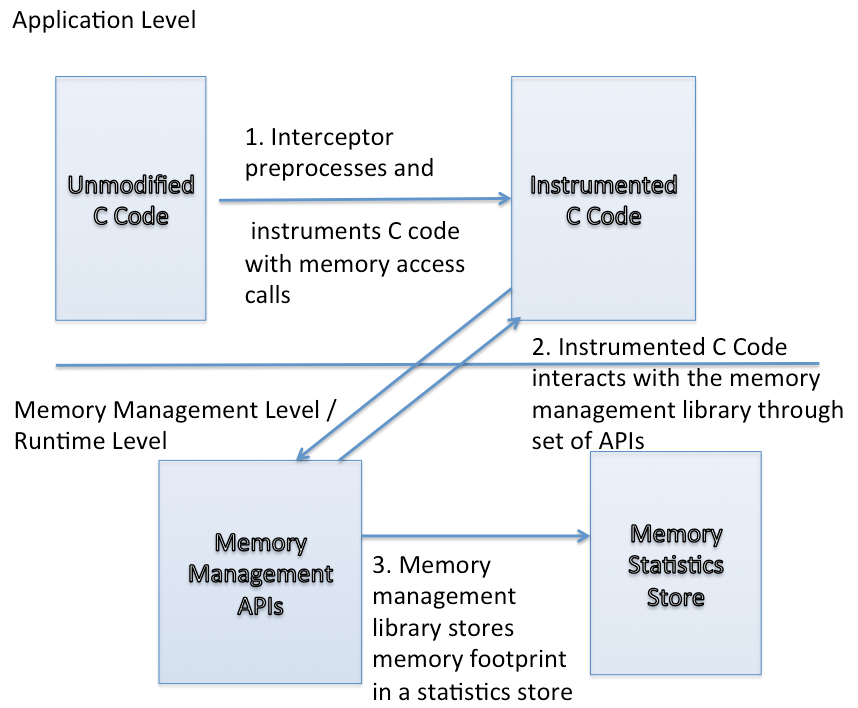
\includegraphics[scale=0.25]{./images/architecture.png}
\end{figure}

\paragraph{Interceptor: Transparent Instrumentation}
The interceptor uses preprocessing and code level instrumentation for injecting calls which enable the monitoring mechanism. In order to monitor object references, Tracer uses an interceptor which pre-processes standard C source code. The interceptor classifies literals into different classes of 8 different class types. {\emph{Identifiers}} allocated as dynamic objects are identified as {\emph{trace targets}}. The interceptor adds an {\emph{access}} function call ({\emph{mem\_access}}) following an access to each {\emph{trace target}}. This {\emph{mem\_access}} library call increments the object's hidden count variable (described in the following section) by one. 
\paragraph{Header Tagged Objects}
Tracer implements a custom version of the standard malloc library function named "{\emph{hmalloc}}" (header memory allocator) which {\emph{transparently}} tags each target object with a header field. The header acts as a custom metadata store for the object. The design philosophy behind tagging objects with headers is to be able to support faster count updates. Our earlier design was plagued by heavy overheads involved in looking up each object's counter within a hash table. {\emph{Object headers}} provide a clean solution to this problem since the metadata is now tagged to each object in memory. {\emph{Hmalloc}} increases the amount of bytes requested by the size of an int, and uses the additional space to store the object count. A pointer to the memory location immediately following these four bytes is then returned to the requesting application. These objects are then added to an object list that Tracer manages, which is a part of the memory statistics store (described below).
\paragraph{Memory Monitoring Interfaces}
We provide the following interface to the application developer for getting memory statistics:
\begin{enumerate}
\item {\emph{void * hmalloc (size\_t bytes)}} - Allocates "bytes" size object tagged with a header.
\item {\emph{void hfree}} - Frees objects tagged with headers.
\item {\emph{void mem\_access\_stat}} - Prints the access count of all the objects allocated by the current program.
\item{\emph{void mem\_access(void *memory\_location, int count)}} - Increases the access count of the object at the memory location (memory\_location) by the count. This function is used by the memory interceptor to monitor access counts at the object-level.
\item {\emph{int mem\_access\_count(void *object\_address)}} - Returns the current access count of the object (at memory location "object\_address").
\end{enumerate}

\begin{figure}
\caption{Binary Tree Benchmark Results For Tree Creation}\label{fig:create}}{%
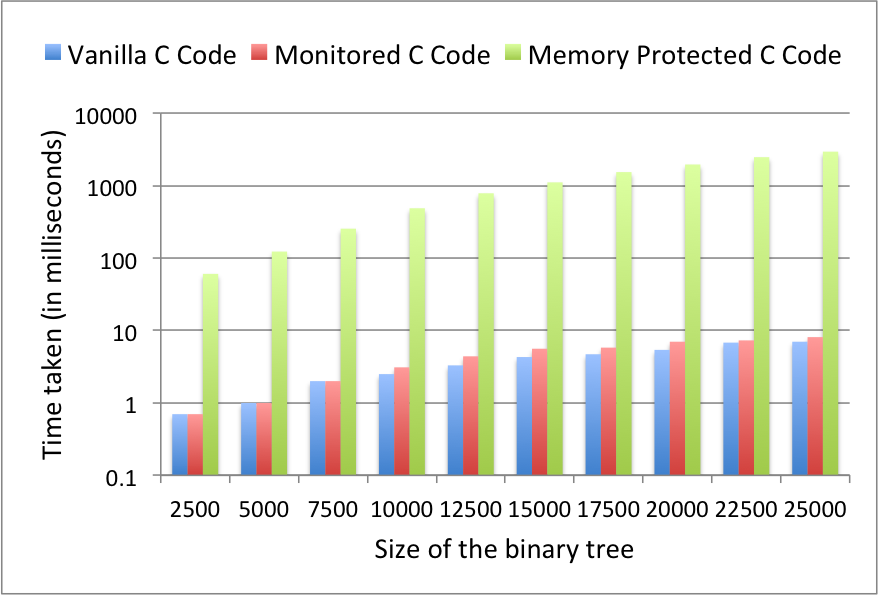
\includegraphics[scale=0.5]{./images/create2.png}  
\end{figure}
